
%%%%%%%%%%%%%%%%% Intro %%%
\section{Introduction}
In this report the spectral analysis of irregularly sampled data - in particular line spectra - is performed using the Fourier Transform. Also, the sparse representation of signals is evaluated by applying different classical methods such as "greedy" algorithms and "convex relaxation" approaches. These methods are applied in particular to irregular sampled data, since this is the most realistic representation of acquired data in astronomy.


%%%%%%%%%%%%%%%%%%%% TASK II %%%%%%%%%%%%%%%%%%%%%%%%%%%
\section{Spectral analysis with Fourier Transform}
\begin{figure}[h!]
	\centering
	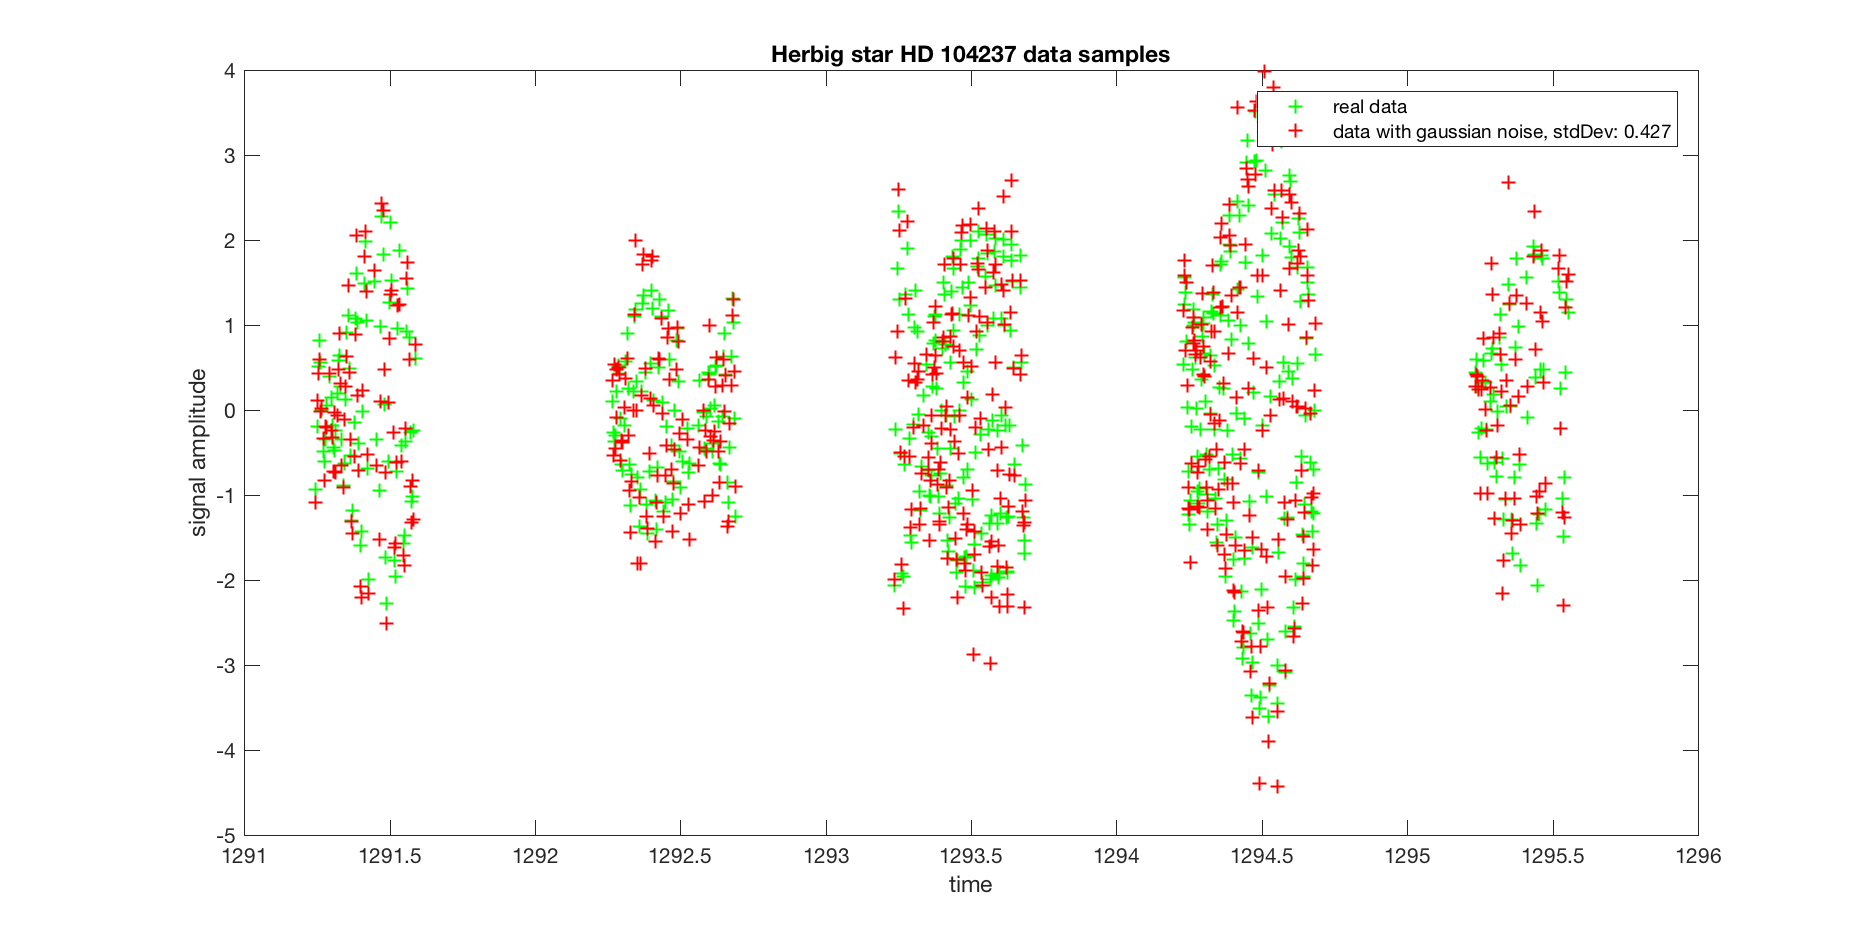
\includegraphics[width=\textwidth]{images/data}
	\caption{Original data samples and samples with additional noise in time domain}
	\label{fig:data}
\end{figure}
Since working on a real data set might be difficult, in particular when it comes to understanding the underlying techniques of the methods aforementioned, we will simulate our irregular sampled data, for which an initial dataset was given (c.f \cref{Appendix A}).
Using this amplitude, phase, time, frequency and the appropriate radial velocity data, the following formula was used to create a realistic data set that is basically a noisy sum of sine functions

\begin{equation}
	\centering
	x(t_n) = \sum_{k=1}^K A_k \sin(2\pi\nu_kt_n + \phi_k) + \epsilon_n
	\label{eq:sinesum}
\end{equation}

As for the Signal-to-Noise ratio 20dB in power mean were used, and for the number of sine functions \texttt{K = 5}, as our initial data set contained 5 different amplitudes and its according phases and frequencies (c.f. \cref{Appendix A}).
\Cref{fig:data} shows the generated data, where the green part corresponds to our simulated data without noise (hereafter seen as "real" or "original" data) and the red part including noise. The noisy data set will be used from here on in all upcoming calculations.



\subsection{Irregular sampling case}
In the case of irregular sampled data we can not apply the Fast-Fourier-Transform (FFT) as we would have in the regular case. However, the Fourier-Transform can be computed by introducing a Matrix $\boldsymbol{W}$, such as
\begin{equation}
	\centering
	\boldsymbol{W}(l,c) = \exp(2j\pi t_l f_c) \quad ,\quad \boldsymbol{\hat{x}} = \boldsymbol{W^\dagger}\boldsymbol{x}
\end{equation}
with $\boldsymbol{\hat{x}}$ being the Fourier-Transform of vector $\boldsymbol{x}$. As stated above, the FFT can not be used here, since the Matrix $\boldsymbol{W}$ must be orthogonal for the FFT - which it is not in the case of irregular sampled data.\\
Nevertheless, having this tool handy, we can now perform the Fourier Transform on irregular sampled data, e.g. on our data set represented in \cref{fig:data}.

\begin{figure}[h!]
	\centering
	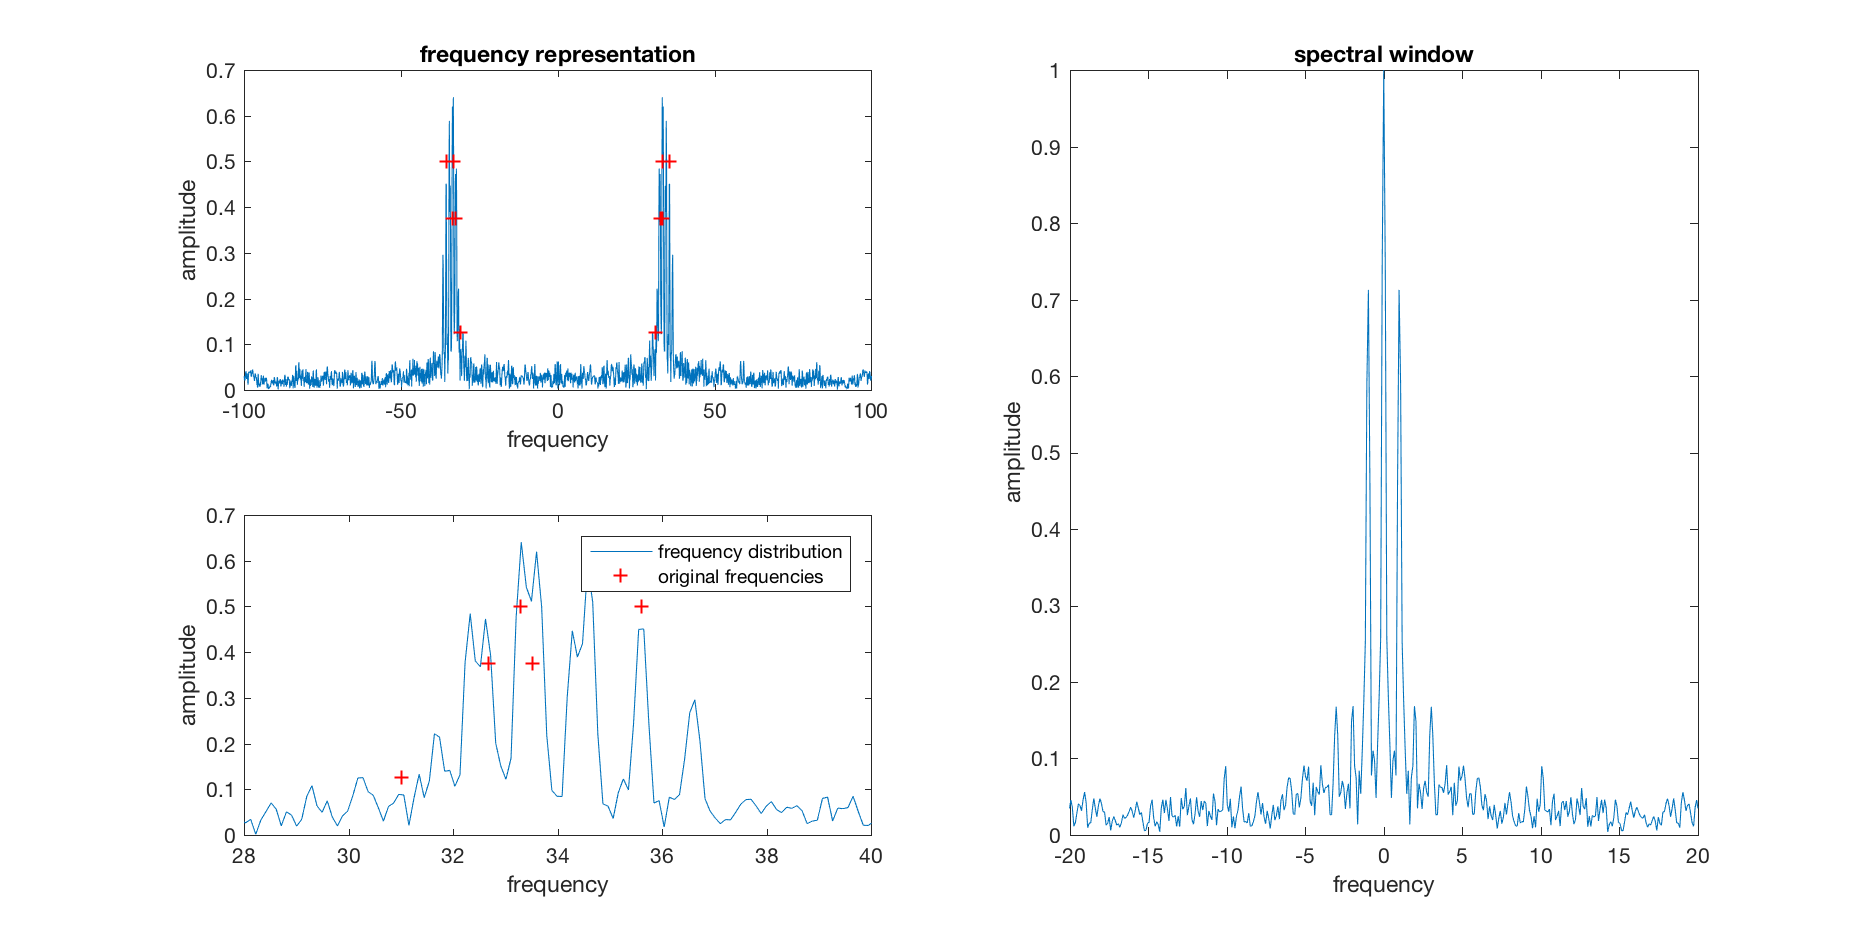
\includegraphics[width=\textwidth]{images/data_freq}
	\caption{Frequency representation with original frequencies and spectral window}
	\label{fig:data_freq}
\end{figure}

For the beginning we only use one sine-function (in \cref{eq:sinesum}, thus \texttt{K=1}). In this case it is very easy to determine the frequency and amplitude of the underlying sine-signal in the frequency representation of data, even if there are quite high side lobes. The phase, which essentially is an offset of the signal, can not be directly read out from the amplitude vs. frequency diagram, but can be calculated from the Fourier-transformed data. The phase will also be affected by the noise intentionally introduced in the data set.\\
However, if a noisy sum of 5 sine signals is used, the underlying frequencies and amplitudes can not be easily determined anymore. This is due to the fact that the sum of signals and their respective noise adds up, so that some peaks might be indistinguishable from others or side lobes. This can be seen in \cref{fig:data_freq} on the left side, where the red cross-hair markings correspond to the original frequency and amplitude, and the blue waveform to the frequency representation of the sum of signals. It is easy to see that the original frequencies and amplitudes can not be read out - only a rough estimation on where the frequencies are located might be is possible by taking into account the location of the highest peaks.

The spectral window corresponding to the sampling time is shown in \cref{fig:data_freq} on the right. The spectral window as represented in the figure shows the Fourier Transform of a rectangular window (basically consisting of $\delta$-functions). The main peak corresponds to the main frequency peak in the frequency domain of the signal - which can be useful in case of truncating specific frequencies or weighting the signal, since the spectral window (in this case similar to a sinc function) can cut off frequencies above the cutoff frequency when convoluted with the Fourier Transformed signal.

The appropriate MATLAB code used to create the initial data set and calculate the frequency representations can be found in \cref{Appendix B}.


%%%%%%%%%%%%%%%%%%%% TASK III %%%%%%%%%%%%%%%%%%%%%%%%%%%
\section{Sparse representation with greedy algorithms}
The framework of sparse representations and greedy algorithms has been invented in order to perform spectral analysis of irregularly sampled data. The idea of such algorithms is to use iterative techniques for signal analysis, i.e. computing the frequency, which maximizes the frequency representation, followed by the subtraction of the related signal from the data and a further frequency analysis based on the resulting data called residual. In this second part, we investigate different algorithms for analysing irregular samples, analyse their performance and compare them. These algorithms are applied to the data set $\boldsymbol{x}$ of 5 signals created in the previous part.
\subsection{Pre-whitening or Matching Pursuit (MP) algorithm}
The general structure of the  Matching Pursuit (MP) algorithm is shown in the Pseudo Code below taken from the laboratory instruction paper. After initialization it searches for the index $k$, for which the frequency representation calculated via $\boldsymbol{\omega}_{k}^{\dag}\boldsymbol{r}_{n}$ is maximized. This can be understood as finding the highest peak in the frequency representation of the signal. Note that in this case $\boldsymbol{\omega}_{k}$ is a column of the spectral window matrix $\boldsymbol{W}$ corresponding to the index $k$. Related to this, we save the chosen indices by listing them in a matrix $\Gamma_n$. The final step in the algorithm then consists of updating the amplitude of the signal corresponding to the frequency related to the index $k$, and finally calculating the residual signal by subtracting this detected signal from the data. The resulting residual data is then used for the following iteration of that algorithm. 

\begin{center}
\fbox{\parbox[c][4cm][t]{12cm}{Initialisation $k=0$, $\boldsymbol{r}_0=\boldsymbol{x}$, $\Gamma_0 = \emptyset$, $\boldsymbol{a}=\boldsymbol{0}$\\
Iterations $n=1 $ . . . \begin{itemize} \item[a)] Select the atom with index $\boldsymbol{k}=\mathrm{arg}\text{ }\mathrm{max}_{k}|\boldsymbol{\omega}_{k}^{\dag}\boldsymbol{r}_{n}|$\\
Update the list of indices $\boldsymbol{\Gamma}_{n}=\boldsymbol{\Gamma}_{n-1}\cup\{k\}$\\

\item[b)] Update the amplitude $a_{k}=a_{k}+\frac{1}{\boldsymbol{\omega}_{k}^{\dag}\boldsymbol{\omega}_{k}}\boldsymbol{\omega}_{k}^{\dag}\boldsymbol{r}_{n}$\\
and the residuals $\boldsymbol{r}_{n}=\boldsymbol{r}_{n-1} - \frac{1}{\boldsymbol{\omega}_{k}^{\dag}\boldsymbol{\omega}_{k}}\boldsymbol{\omega}_{k}^{\dag}\boldsymbol{r}_{n}\boldsymbol{\omega}_{k}$

\end{itemize}
}
}
\end{center}
One has to choose a stopping rule for that algorithm, as well. We can assume that after a certain amount of iteration steps the residual $\boldsymbol{r}$ only consists of Gaussian noise, since most of the real signal was detected and reduced from the data at that point. Therefore, the remaining data in $\boldsymbol{r}$ consists of centered Gaussian noise with variance $\sigma^{2}$, which is known. The variable defined by $T=\frac{||\boldsymbol{r}||^{2}}{\sigma^{2}}$ has a $\chi^{2}$ distribution with $N$ degrees of freedom. We stop the algorithm as soon as $T<\tau$ is given for the case that the probability for that is given by $P(T < \tau)=0.95$.

Our implementation of that algorithm in MATLAB is presented in the code in the appendix. The resulting diagrams are shown in figure \ref{fig:mp}. The upper panel displays the frequency representation of the analysed signal, plotting the amplitude for the detected frequency, while the lower panel is the inverse fourier transfor of the upper panel, thus showing the actual result of the analysis in time space. In addition, the upper panel displays the comparison between the analysed frequencies and the actual amplitudes and frequencies within the actual used signal data.

\begin{figure}[!h]
	\centering
		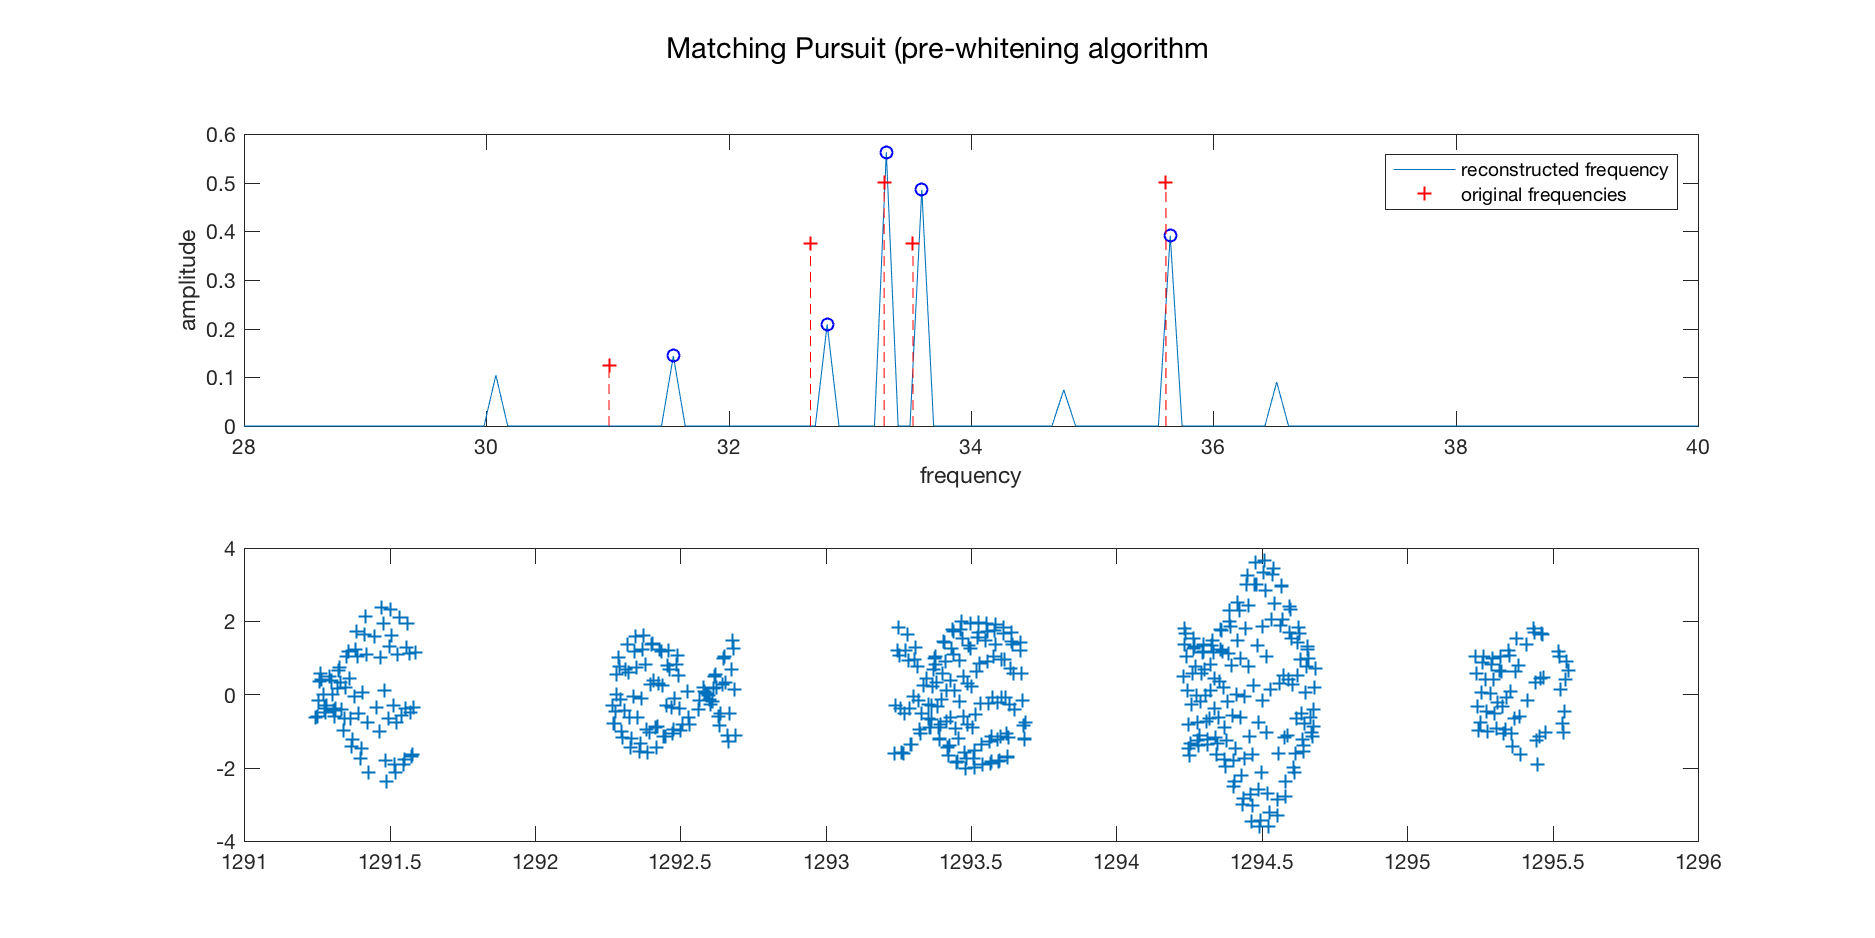
\includegraphics[width=\textwidth]{images/mp}
		\caption{The upper panel shows a comparison between the analysis result using MP-algorithm and the actual signal data in frequency representation, the lower panel displays the signal resulting from the MP algorithm in time domain}
		\label{fig:mp}
\end{figure}

Already in this plot one can observe that this matching point algorithm detects 10 frequencies, although the original signal contained only 5. In addition, the location of those frequencies is detected with small deviations only for the signals with the highest amplitudes.  For the other frequencies the location is not detected correctly. There are also deviations from the original signals concerning the amplitudes of the signals. Table \ref{tab:mp} lists the results of the signal analysis using the MP algorithm together with the specification of the original input signal. Note that in the plots and the table we only consider the absolute values of the frequencies and also ignore the false detections in the table, which is only used to illustrate the precision of the algorithm with respect to the original data.

\begin{table}[h!]
\centering
\begin{tabular}{ | c| c| c| c| c| c|c|c| }
\hline
	&   & Signal 1 & Signal 2 & Signal 3 & Signal 4 & Signal 5 \\ \hline
\multirow{2}{3cm}{Input signal} & Frequency [day$^{-1}$] & 31.012 & 32.675 & 33.283 & 33.521 & 35.609 \\ \cline{2-7}
 & Amplitude & 0.125 & 0.375 & 0.5 & 0.375 & 0.5 \\ \hline

\multirow{2}{3cm}{MP output} & Frequency [day$^{-1}$] &  31.543& 32.812 & 33.301 & 33.594 & 35.645 \\ \cline{2-7}
 & Amplitude &  0.144& 0.209& 0.563 & 0.486 & 0.391 \\ \hline

\end{tabular}
\caption{Parameter comparison ignoring the additional signals found by the MP algorithm}
\label{tab:mp}
\end{table}

Despite the actual performance regarding results, one also has to consider the performance of the algorithm during the signal analysis. An indicator for this is the number of iteration steps before the algorithm converges and stops, which is 38 in the case of this matching pursuit algorithm implementation. During those 38 iteration steps, several indices $k$ reappaeared and were analysed again, which is one main drawback of that method.

% iterations: 56



\subsection{Orthogonal Matching Pursuit (OMP) algorithm}
The drawback of repeating the analysis of several atoms in the matching pursuit algorithm implemented in the previous step can be overcome by using the orthogonal matching pursuit (OMP) algorithm, which updates the amplitudes of all atoms corresponding to indices $k$. Therefore, an orthogonal projection of the data onto the atoms is required, given by the following relation: 
\begin{equation}
\boldsymbol{a}\left(\Gamma_{n}\right)= \underset{\boldsymbol{a}\left(\Gamma_{n}\right)}\argmin || \boldsymbol{x}- \boldsymbol{W}_{\Gamma_{n}}\boldsymbol{a}\left(\Gamma_{n}\right) ||^{2}=\left(\boldsymbol{W}_{\boldsymbol{\Gamma}_{n}}^{\dag}\boldsymbol{W}_{\boldsymbol{\Gamma}_{n}}\right)^{-1}\boldsymbol{W}_{\boldsymbol{\Gamma}_{n}}^{\dag}\boldsymbol{x}
\label{eq:omp}
\end{equation}
In this equation, $\boldsymbol{a}\left(\Gamma_{n} \right)$ are the components of $\boldsymbol{a}$  with all indices $\Gamma_{n}$, while the matrix $\boldsymbol{W}_{\Gamma_{n}}$ is a matrix that is extracted from the original matrix $\boldsymbol{W}$ and contains the columns of that matrix with indices $\Gamma_{n}$.  Using that formalism, the amplitudes are saved or updated for all indices $\Gamma_{n}$ used before or detected in the current step. Thus, the step b) of the matching pursuit algorithm has to be changed accordingly by replacing the calculation of individual amplitudes $\alpha_{k}$ with the calculation of a whole vector $\boldsymbol{\alpha}\left(\Gamma_{n}\right)$ via equation \ref{eq:omp}, as well as the calculation of the residuals, which can now be performed using $\boldsymbol{r}_{n}=\boldsymbol{x}-\boldsymbol{W}_{\Gamma_{n}}\boldsymbol{a}\left(\Gamma_{n}\right)$, has to be replaced. \\
It is important to understad the difference in the calculation of the residuals compared to the previous matching algorithm, because it is now sufficient to subtract the current analysed signal in each step, which gets updated at each step by keeping track of the already analysed and detected indices $\Gamma_{n}$,  from the complete original data set $\boldsymbol{x}$. The final result of an example run of the OMP is presented in figure \ref{fig:omp}, again comparing the original data and the analysed signal in frequency domain in the upper panel and the result of the analysis algorithm in time space in the lower panel. In addition, the extracted data set is quantitatively compared to the original signals in table \ref{tab:omp} ignoring additional false detections.

\begin{figure}[H]
	\centering
		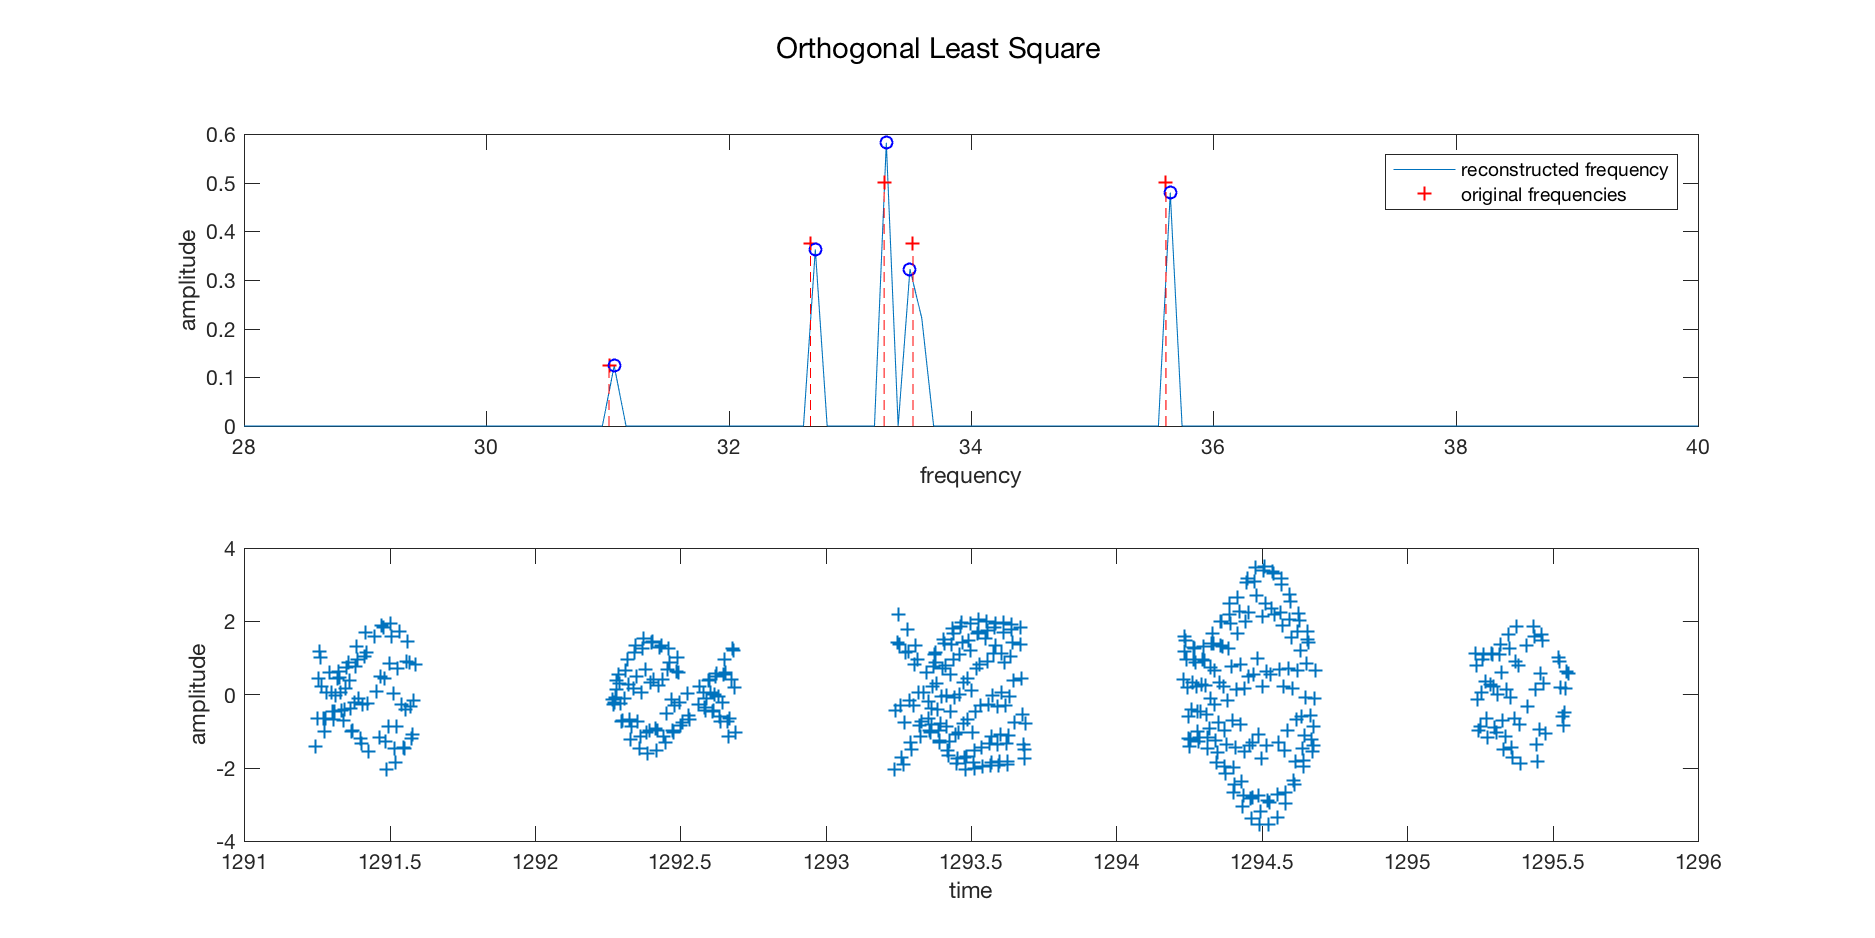
\includegraphics[width=\textwidth]{images/omp}
		\caption{The upper panel shows a comparison between the analysis result using OMP-algorithm and the actual signal data in frequency representation, the lower panel displays the signal resulting from the OMP algorithm in time domain.}
		\label{fig:omp}
\end{figure}

In the case of this OMP, one can see that, in comparison to the MP algorithm, there are less false detected signals, i.e. 8 signals are resulting in total instead of 10, which already is an improvement of the algorithm. Also the estimation of the location of the actual frequencies in the signal has a tendency to be better than before, but still is incorrect for several frequencies and especially for the smallest one. Just by comparing the frequency location of the signals in the data compared to the location of the frequencies resulting from the analysis one can see a deviation. Furthermore, the amplitudes are not correctly estimated for most of the frequencies. However, an advantage of the OMP is the number of necessary iteration steps to achieve those results, which was reduced by more than a factor of two to 16 steps, because the algorithm keeps track of already used indices, reducing the calculation time.

\begin{table}[H]
\centering
\begin{tabular}{ | c| c| c| c| c| c|c|c| }
\hline
	&   & Signal 1 & Signal 2 & Signal 3 & Signal 4 & Signal 5 \\ \hline
\multirow{2}{3cm}{Input signal} & Frequency [day$^{-1}$] & 31.012 & 32.675 & 33.283 & 33.521 & 35.609 \\ \cline{2-7}
 & Amplitude & 0.125 & 0.375 & 0.5 & 0.375 & 0.5 \\ \hline

\multirow{2}{3cm}{OMP output} & Frequency [day$^{-1}$] & 31.738  & 32.812 & 33.301 & 33.594  & 35.645  \\ \cline{2-7}
 & Amplitude & 0.139 & 0.156 & 0.544  & 0.539  & 0.390 \\ \hline

\end{tabular}
\caption{Parameter comparison ignoring the additional signals found by the OMP algorithm.}
\label{tab:omp}
\end{table}


%iterations: 22

\subsection{Orthogonal Least Square (OLS)}
The previous algorithms made use of the matrix $\boldsymbol{W}$ in order to calculate the Fourier transform using the FFT and also the inverse. However, this requires for the matrix $\boldsymbol{W}$ to be orthogonal with $\boldsymbol{W}^{\dag}\boldsymbol{W}=N\boldsymbol{I}$. In the case of irregularly sampled data like our data, that property is not given, which was ignored by the previous algorithms leading to the observed inaccuracies. The Orthogonal Least Square algorithm (OLS) corrects the OLP for that by replacing the selection step a) with the selection of index $k$, for which the approximation error is minimzed when adding the column $\boldsymbol{\omega}_{k}$ to $\boldsymbol{W}_{\Gamma_{n}}$. This optimization is formulated as a least square minimisation via:

\begin{equation*}
k=\underset{k}\argmin\text{ } \underset{\boldsymbol{a}\left(\Gamma_{n}\cup\left(k\right)\right)}\argmin ||\boldsymbol{x} - \boldsymbol{W}_{\Gamma_{n}\cup \{k\}}\boldsymbol{a}\left( \Gamma_{n}\cup \{k\}\right)  ||^{2}
\end{equation*}
Since a non-optimal implementation of such an algorithm can result in a long computing time, we use the matlab function \texttt{ols}: \texttt{[a, ind]= ols(W,x,Inf,test)}. As test for the stop criterium \texttt{test}$=\sigma_{b}^{2}\tau$  is used. This method is implemented in the code shown in the appendix, as well. Also, the comparisons of the signal data to the signal resulting from the analysis using the OLS method are listed in table \ref{tab:ols} and displayed in figure \ref{fig:ols} in analogy to the previous algorithms. 

\begin{table}[h!]
\centering
\begin{tabular}{ | c| c| c| c| c| c|c|c| }
\hline
	&   & Signal 1 & Signal 2 & Signal 3 & Signal 4 & Signal 5 \\ \hline
\multirow{2}{3cm}{Input signal} & Frequency [day$^{-1}$] & 31.012 & 32.675 & 33.283 & 33.521 & 35.609 \\ \cline{2-7}
 & Amplitude & 0.125 & 0.375 & 0.5 & 0.375 & 0.5 \\ \hline

\multirow{2}{3cm}{OLS output} & Frequency [day$^{-1}$] &31.055  & 32.715 & 33.301 & 33.496  & 35.645  \\ \cline{2-7}
 & Amplitude & 0.114 & 0.327 & 0.549  & 0.293  & 0.376 \\ \hline

\end{tabular}
\caption{Parameter comparison ignoring the additional signals found by the OLS algorithm.}
\label{tab:ols}
\end{table}

\begin{figure}[H]
	\centering
		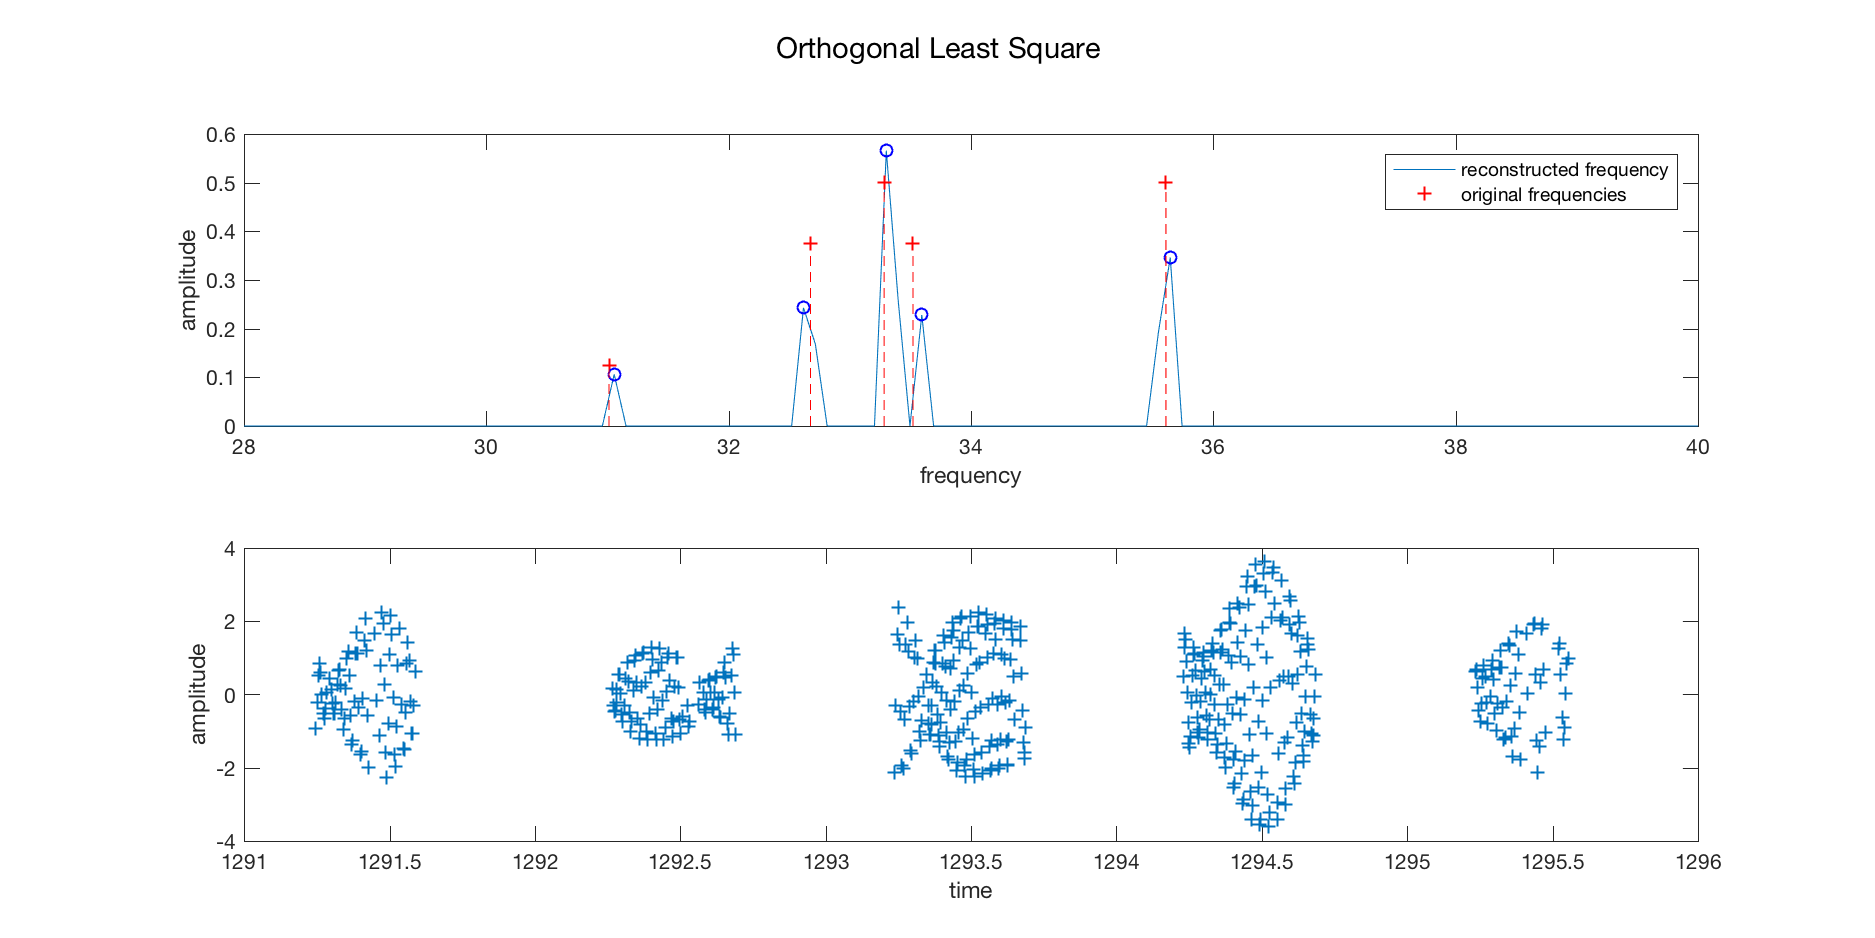
\includegraphics[width=\textwidth]{images/ols}
		\caption{The upper panel shows a comparison between the analysis result using the OLS-algorithm and the actual signal data in frequency representation, the lower panel displays the signal resulting from the OLS algorithm in time domain.}
		\label{fig:ols}
\end{figure}

The OLS algorithm does not show any false detections, and also the locations of the 5 frequencies in the original data set are obtained correctly. Also the amplitudes of each of the detected signals are correctly estimated for at least 3 of the 5 signals, while the difference between the estimated amplitude and original amplitude for the remaining two signals is relatively small. Also, the number of iteration steps is relatively low with only 13 required steps. This result shows how the OLS is a strong improvement of the previous two algorithms.



% iterations: 22


%%%%%%%%%%%%%%%%%%%% TASK IV %%%%%%%%%%%%%%%%%%%%%%%%%%%
\section{Sparse representation with convex relaxation}
Instead of using matching pursuit algorithms for obtaining a sparse representation, one can also minimize a convex quadratic cost function including a $l^{1}$-norm, as given in equation \ref{eq:convex}:
\begin{equation}
\boldsymbol{a}=\underset{\boldsymbol{a}}\argmin ||\boldsymbol{x} - \boldsymbol{Wa} ||^{2} +\lambda ||\boldsymbol{a}||_{l} \text{ with } ||\boldsymbol{a}||_{l} =\sum_{k}|\boldsymbol{a}_{k} |
\label{eq:convex}
\end{equation}
For using that as a minimzing algorithm, we make use of the matlab function \texttt{min\_12\_11\_0}. The amplitude vector $\boldsymbol{a}$ can be calculated with \texttt{min\_12\_11\_0(x,W,lambda,n\_it\_max)}, where the number of iteration steps for the algorithm \texttt{n\_it\_max} has to be defined. In general, the solution satisfies the condition $|\boldsymbol{W}^{\dag}\left(\boldsymbol{x}-\boldsymbol{Wa} \right)| \leq\lambda $. Because of that, $\lambda$ is the actual parameter describing the accuracy of the fit by stating that the frequency representation of the residual in the case that the convergence is smaller than $\frac{\lambda}{N}$. Therefore, $\lambda$ has to be tuned in order to find a satisfying solution. In our case, $\lambda $ is chosen to be 6\% of the maximum of the frequency representation of the residual, and a maximum number of iteration steps of $n_{it,max}= 100000$ is applied. In those cases, the algorithm presents a solution within a reasonable computation time. Our implementation of the code is again given in the MATLAB code in the appendix and the results are again shown in figure \ref{fig:convex} and listed in table \ref{tab:convex}.\\
The convex relaxation algorithm also does not show a lot of false detections, i.e. only 3 with very low amplitude, which only result from the very accurate stopping rule that we used with the small $\lambda$. These false detections could actually be caused by a frequent pattern in the noise of the data. However, it has a good accuracy in detecting the location of the frequencies, although it is not able to reconstruct the correct amplitudes for almost all of the signals.


\begin{table}[h!]
\centering
\begin{tabular}{ | c| c| c| c| c| c|c|c| }
\hline
	&   & Signal 1 & Signal 2 & Signal 3 & Signal 4 & Signal 5 \\ \hline
\multirow{2}{3cm}{Input signal} & Frequency [day$^{-1}$] & 31.012 & 32.675 & 33.283 & 33.521 & 35.609 \\ \cline{2-7}
 & Amplitude & 0.125 & 0.375 & 0.5 & 0.375 & 0.5 \\ \hline

\multirow{2}{3cm}{OLS output} & Frequency [day$^{-1}$] &30.957  & 32.715 & 33.301 & 33.496  & 35.645  \\ \cline{2-7}
 & Amplitude & 0.032 & 0.158 & 0.454  & 0.193  & 0.314 \\ \hline

\end{tabular}
\caption{Parameter comparison ignoring the additional signals found by the convex relaxation algorithm}
\label{tab:convex}
\end{table}


\begin{figure}[!h]
	\centering
		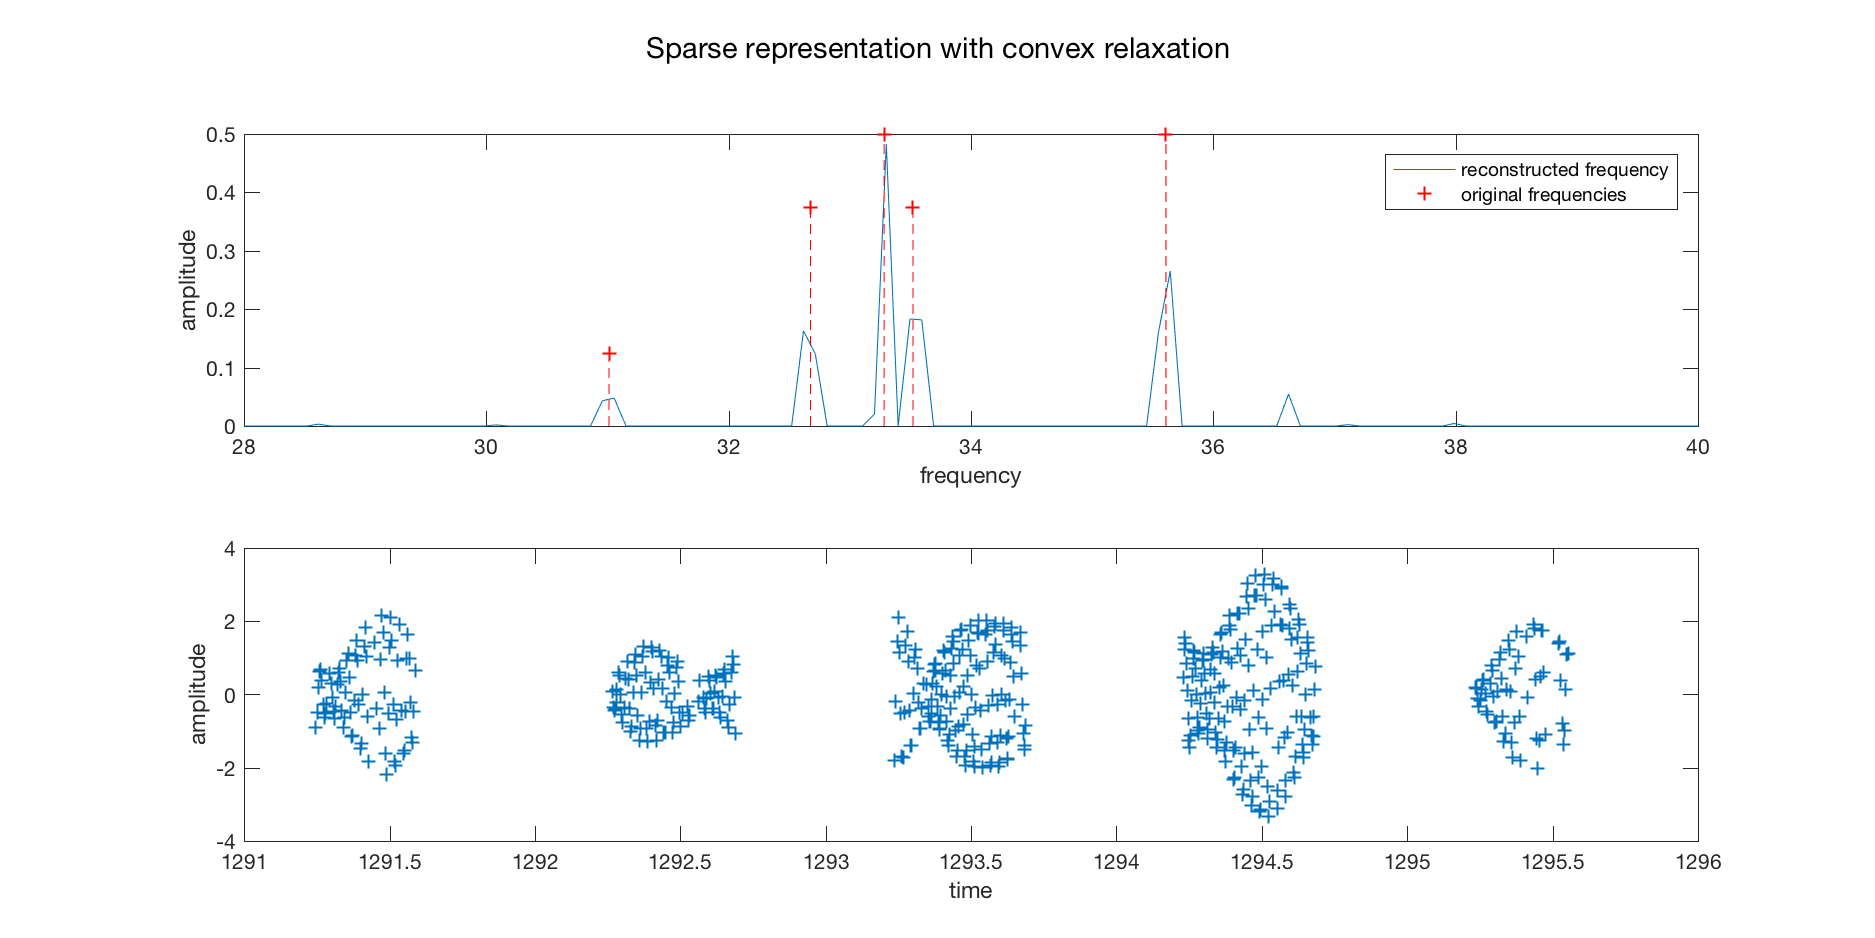
\includegraphics[width=\textwidth]{images/convex}
		\caption{The upper panel shows a comparison between analysis result using the convex relaxation-algorithm and the actual signal data in frequency representation, the lower panel displays the signal resulting from the convex relaxation algorithm in time domain}
		\label{fig:convex}
\end{figure}

%lambdamax:331.2451, used: 0.05*lambdamax


%%%%%%%%%%%%%%%%%%%%%%%%%%%%%CONCLUSION%%%%%%%%%%%%%%%%%%%%%%%%%%%%%%%
\section{Conclusion}
In this report, the spectral analysis of irregular sampled data, i.e. line spectra, was analysed. In a first step, a corresponding data set including 5 different signals of different frequency and amplitudes, as well as a random noise component, was constructed and fourier transformed using a spectral window matrix $\boldsymbol{W}$. In the second part, several different greedy algorithms were applied to obtain the sparse representation of that data set. The first basic matching pursuit algorithm showed a lot of false detections, inaccurate frequency and amplitude detection. The improved orthogonal matching pursuit algorithm especially reduced the number of iteration steps required before convergence, but still was not robust against false detections. Furthermore, it also did not detect the location and amplitude of the actual signals precisely. However, the orthogonal least square algorithm showed the best performance of the used algorithms with a relatively short computation time, robustness to false detection and a very accurate detection of frequencies and their amplitudes. The finally tested convex relaxation method also only showed a few false detections and a good performance regarding the detection of location of the frequencies. But in doing so it required a very long computation time. As a conclusion, in the case of irregularly sampled data we recommend to use the orthognal least square method, since it is robust and accurate, with a reasonably limited computation time.
